\begin{frame}{Traction Control}
\framesubtitle{Gray Box Model}
\resizebox{\textwidth}{!}{%
\begin{tikzpicture}[auto, node distance=2cm,>=latex']
    % We start by placing the blocks
    \node [sum] (sum) {};
    \node [input, left of = sum, yshift = 1cm] (vr) {};
    \node [input, left of = sum, yshift = -1cm](vl) {};
    \node [sum, right of = sum, xshift = 1cm](addspeedsetpoint){};
    \node [input, below of = addspeedsetpoint](speed0){};
    \node [block, right of = addspeedsetpoint, xshift = 1cm](strip){$Trac(s)?$};
    \node [sum, right of = strip, xshift = 2cm](addtracsetpoint){};
    \node [input, below of = addtracsetpoint](tracsetpoint){};
    \node [output, right of = addtracsetpoint](trac){};

    % Once the nodes are placed, connecting them is easy.
    \draw [draw,->] (vr) node [yshift = 3mm]{$\omega_R$} -| node [pos = 0.9]{$+$} (sum);
    \draw [draw,->] (vl) node [yshift = 3mm]{$\omega_L$} -| node [pos = 0.9]{$-$} (sum);
    \draw [draw,->] (sum) -- node {$\Delta_\omega$} node[pos = 0.9]{$+$}  (addspeedsetpoint);
    \draw [draw,->] (speed0) -- node{${\Delta_\omega}_0$} node [pos = 0.9, right]{$-$} (addspeedsetpoint);
    \draw [draw,->]  (addspeedsetpoint) -- node{${\tilde{\Delta_\omega}}$} (strip);
    \draw [draw,->] (strip) -- node {$\tilde{f}$} node[pos = 0.9]{$+$} (addtracsetpoint);
    \draw [draw,->] (tracsetpoint) -- node {$f_0$} node[pos = 0.9, right]{$+$} (addtracsetpoint);
    \draw [draw,->] (addtracsetpoint) -- node {$f$} (trac);

\end{tikzpicture}}
\end{frame}

\begin{frame}{Traction Control}
\framesubtitle{Gray Box Model -- Refined}
\resizebox{\textwidth}{!}{%
\begin{tikzpicture}[auto, node distance=2cm,>=latex']
    % We start by placing the blocks
    \node [input](input){};
    \node [sum, right of = input, xshift = 0.5cm](add){};
    \node [input, above of = add, yshift = -0.8cm](disturb){};
    \node [square, right of = add, xshift = 0cm](integrator){$\frac{1}{s}$};
    \node [block, right of = integrator, xshift = 2.5cm](strip){$H(s)?$};
    \node [output, right of = strip](trac){};

    % Once the nodes are placed, connecting them is easy.
    \draw [draw,->]  (input) -- node{${\tilde{\omega_L}}$} node[pos = 0.9, below]{$-$} (add);
    \draw [draw,->]  (disturb) -- node[pos = 0.2]{$d$} node[pos = 0.9]{$+$} (add);
    \draw [draw,->]  (add) -- (integrator);
    \draw [draw,->]  (integrator) -- node{${\int^t_0\tilde{\omega_L}}dt$} (strip);
    \draw [draw,->] (strip) -- node {$\tilde{f}$} (trac);
\end{tikzpicture}}
\end{frame}

\begin{frame}
\[Trac(s) = 13.096\cdot\frac{s+0.9221}{s(s+4.063)}\]
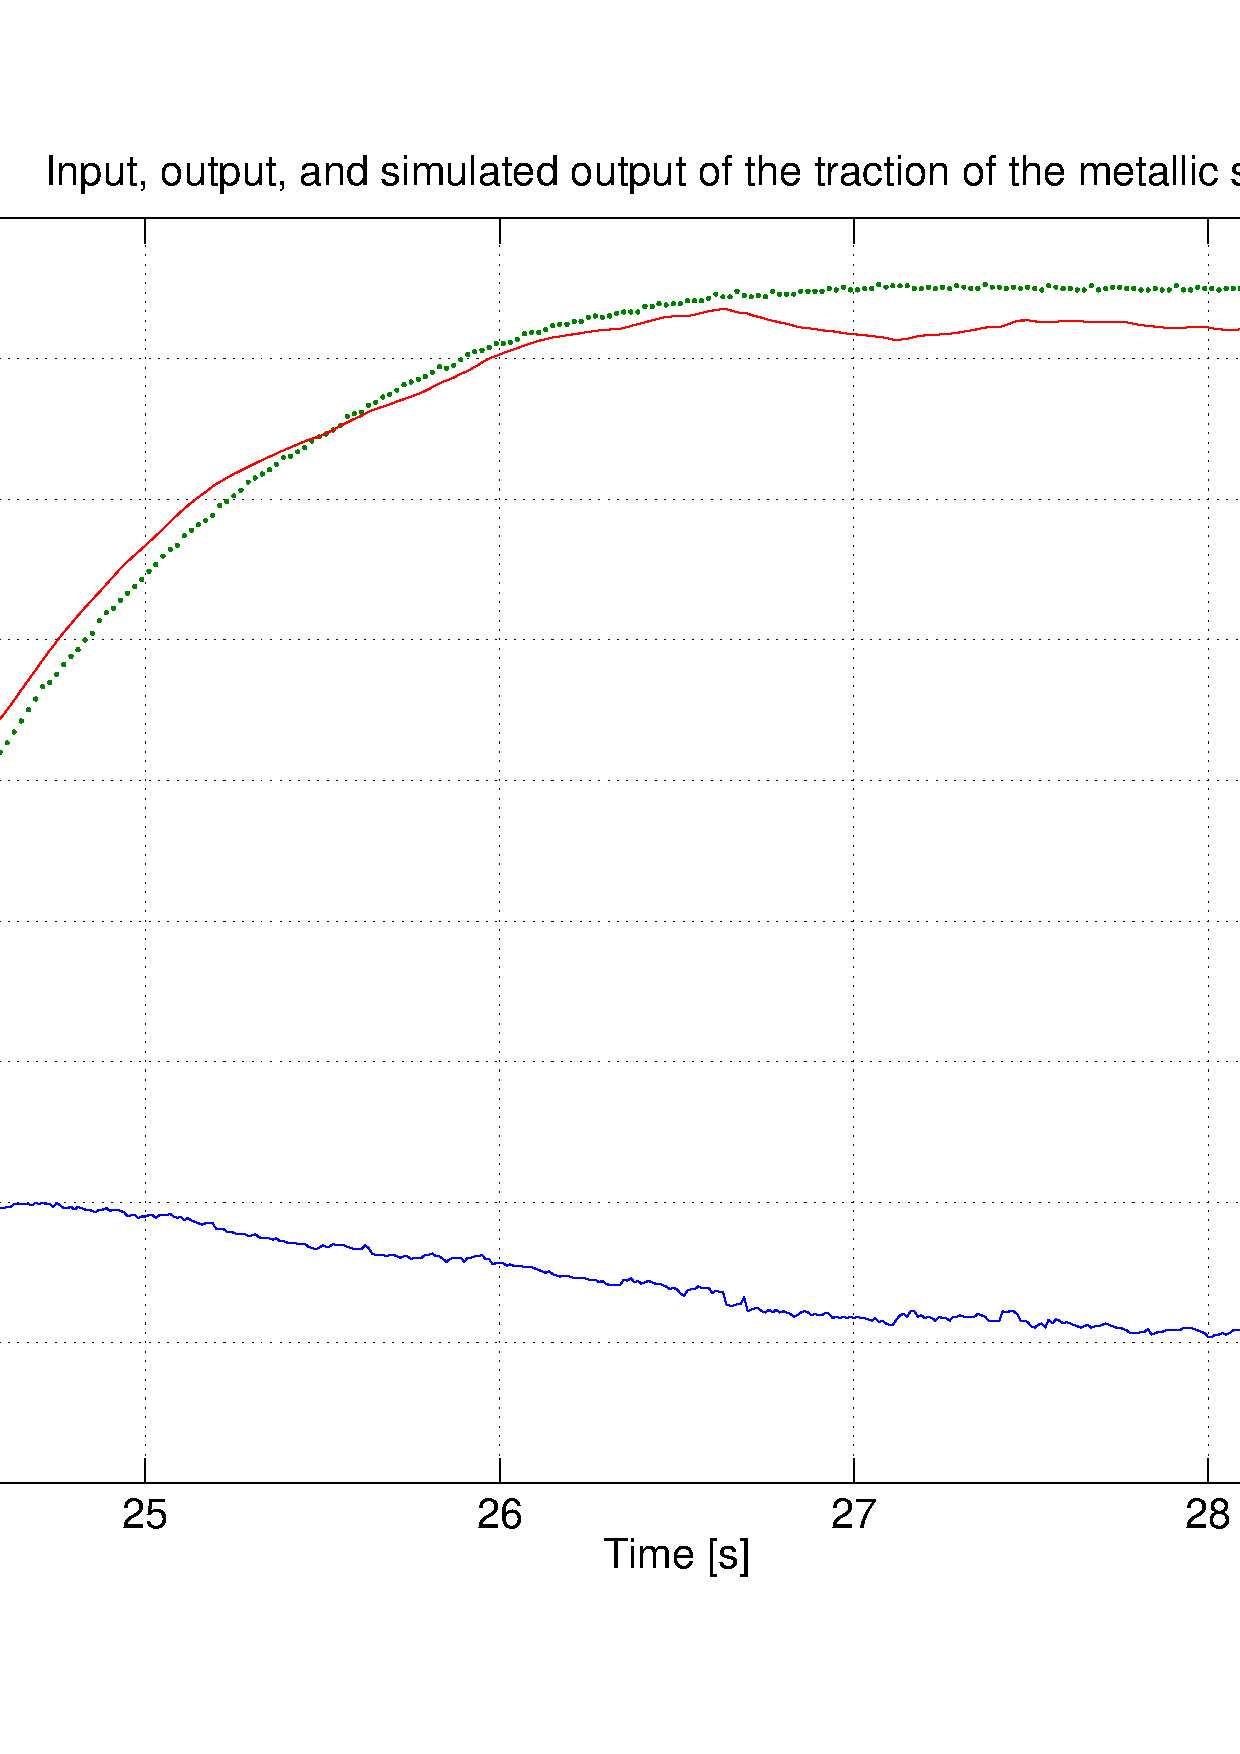
\includegraphics[width = \textwidth]{tracFit.pdf}
\end{frame}

\begin{frame}{Traction Control}
\framesubtitle{Controller Choice}
\begin{block}{First tentative: simple P controller}
\begin{itemize}
\item Integrator in the plant should provide zero steady state error
\item Added integrator would degrade the phase margin
\item No specification on the transient
\end{itemize}
\end{block}
\end{frame}

\begin{frame}{Traction Control}
\centering
\framesubtitle{Simulation -- Simple P Controller}
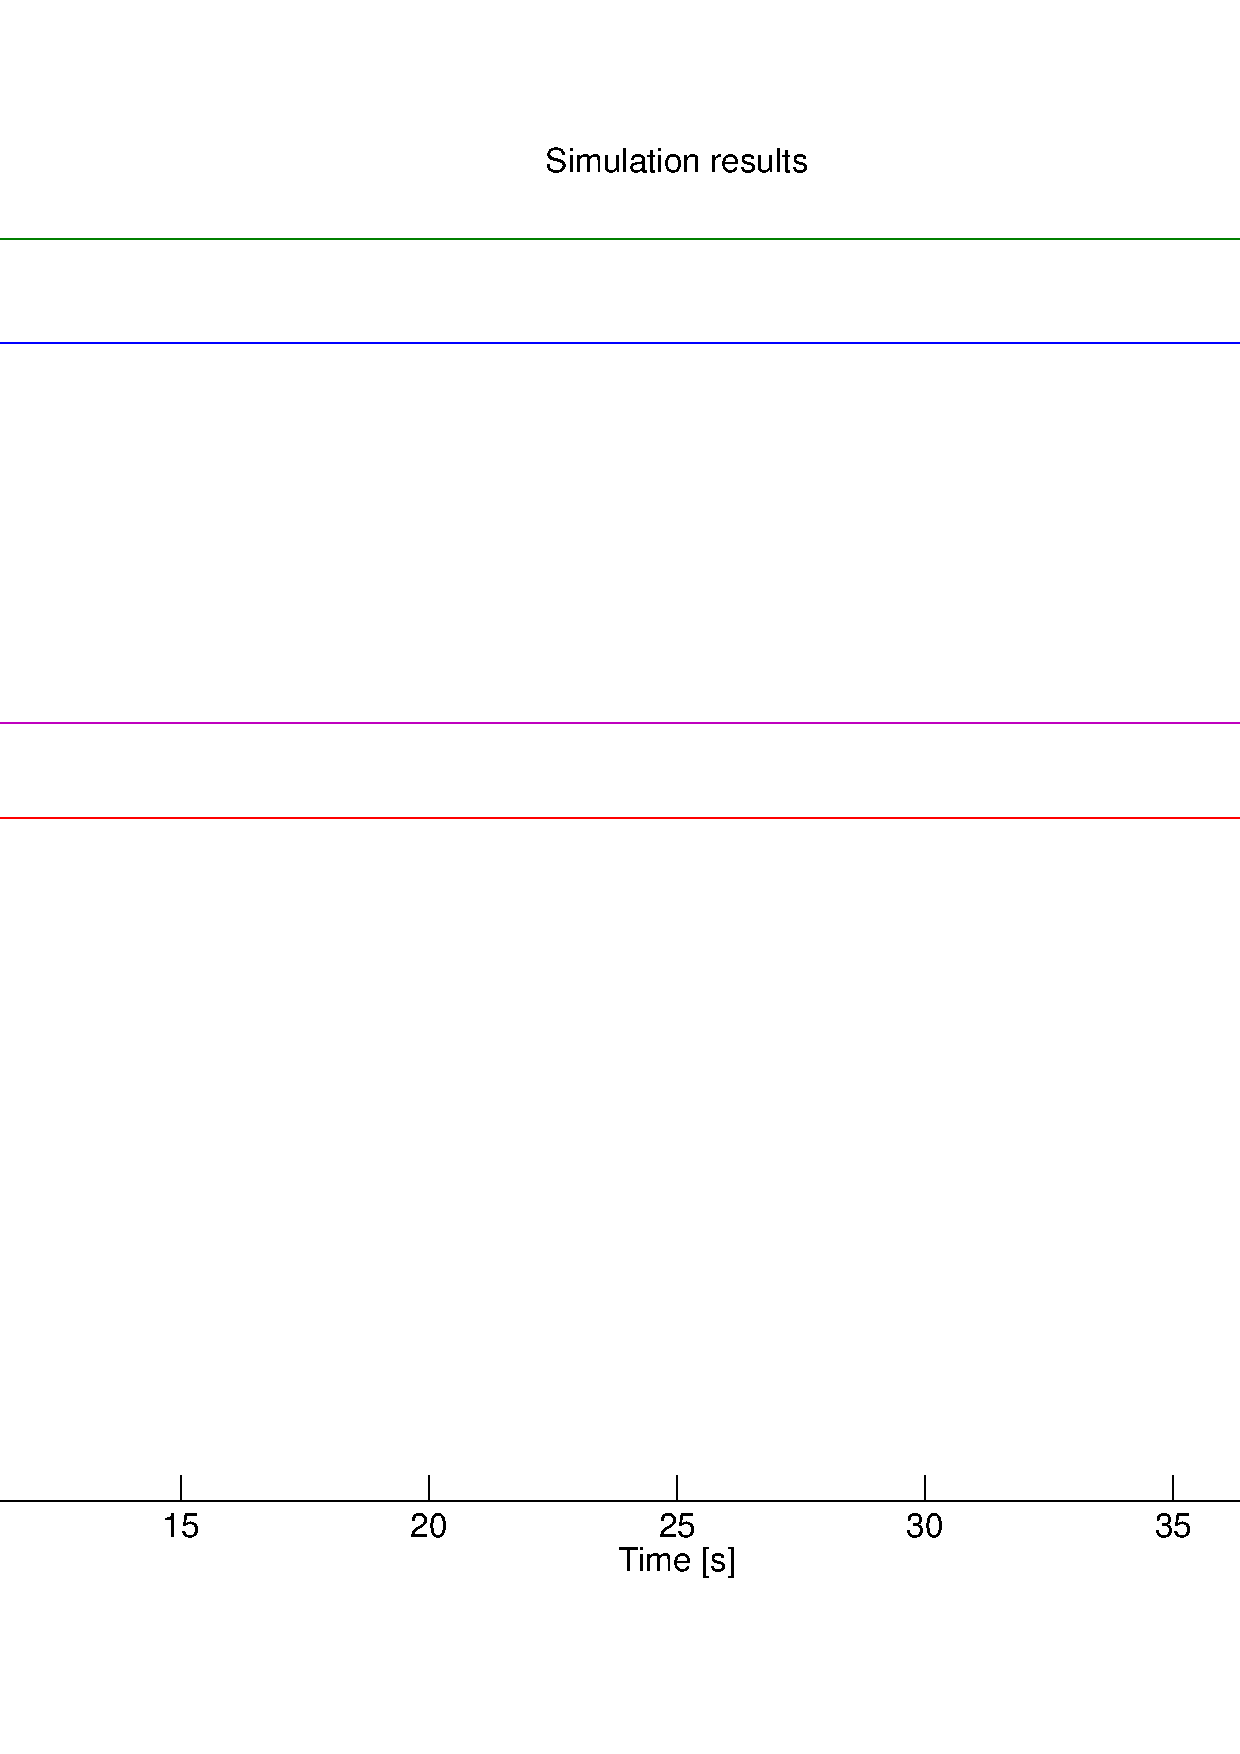
\includegraphics[width = \textwidth]{simu_P_tot.pdf}
\end{frame}

\begin{frame}{Traction Control}
\framesubtitle{Controller Choice}
\begin{itemize}
\item Steady state error is due to perturbation from the master speed, constant in regime
\item Simple P controller
\\$\Rightarrow$ No perturbation rejection
\\$\Rightarrow$ But removes integrator from the closed loop!
\item Idea: second outer PI loop to reject the constant perturbation
\item Possible in terms of phase margin thanks to the inner P controller
\end{itemize}
\end{frame}

\begin{frame}{Traction Control}
\framesubtitle{Final Controller}
\includegraphics[width = 1.05\textwidth]{simulink.png}
\end{frame}

\begin{frame}{Traction Control}
\framesubtitle{Controller Tuning -- Inner Traction Loop}
\includegraphics[width = \textwidth]{rmTrac_locus.pdf}
\end{frame}

\begin{frame}{Traction Control}
\framesubtitle{Controller Tuning -- Outer Traction Loop}
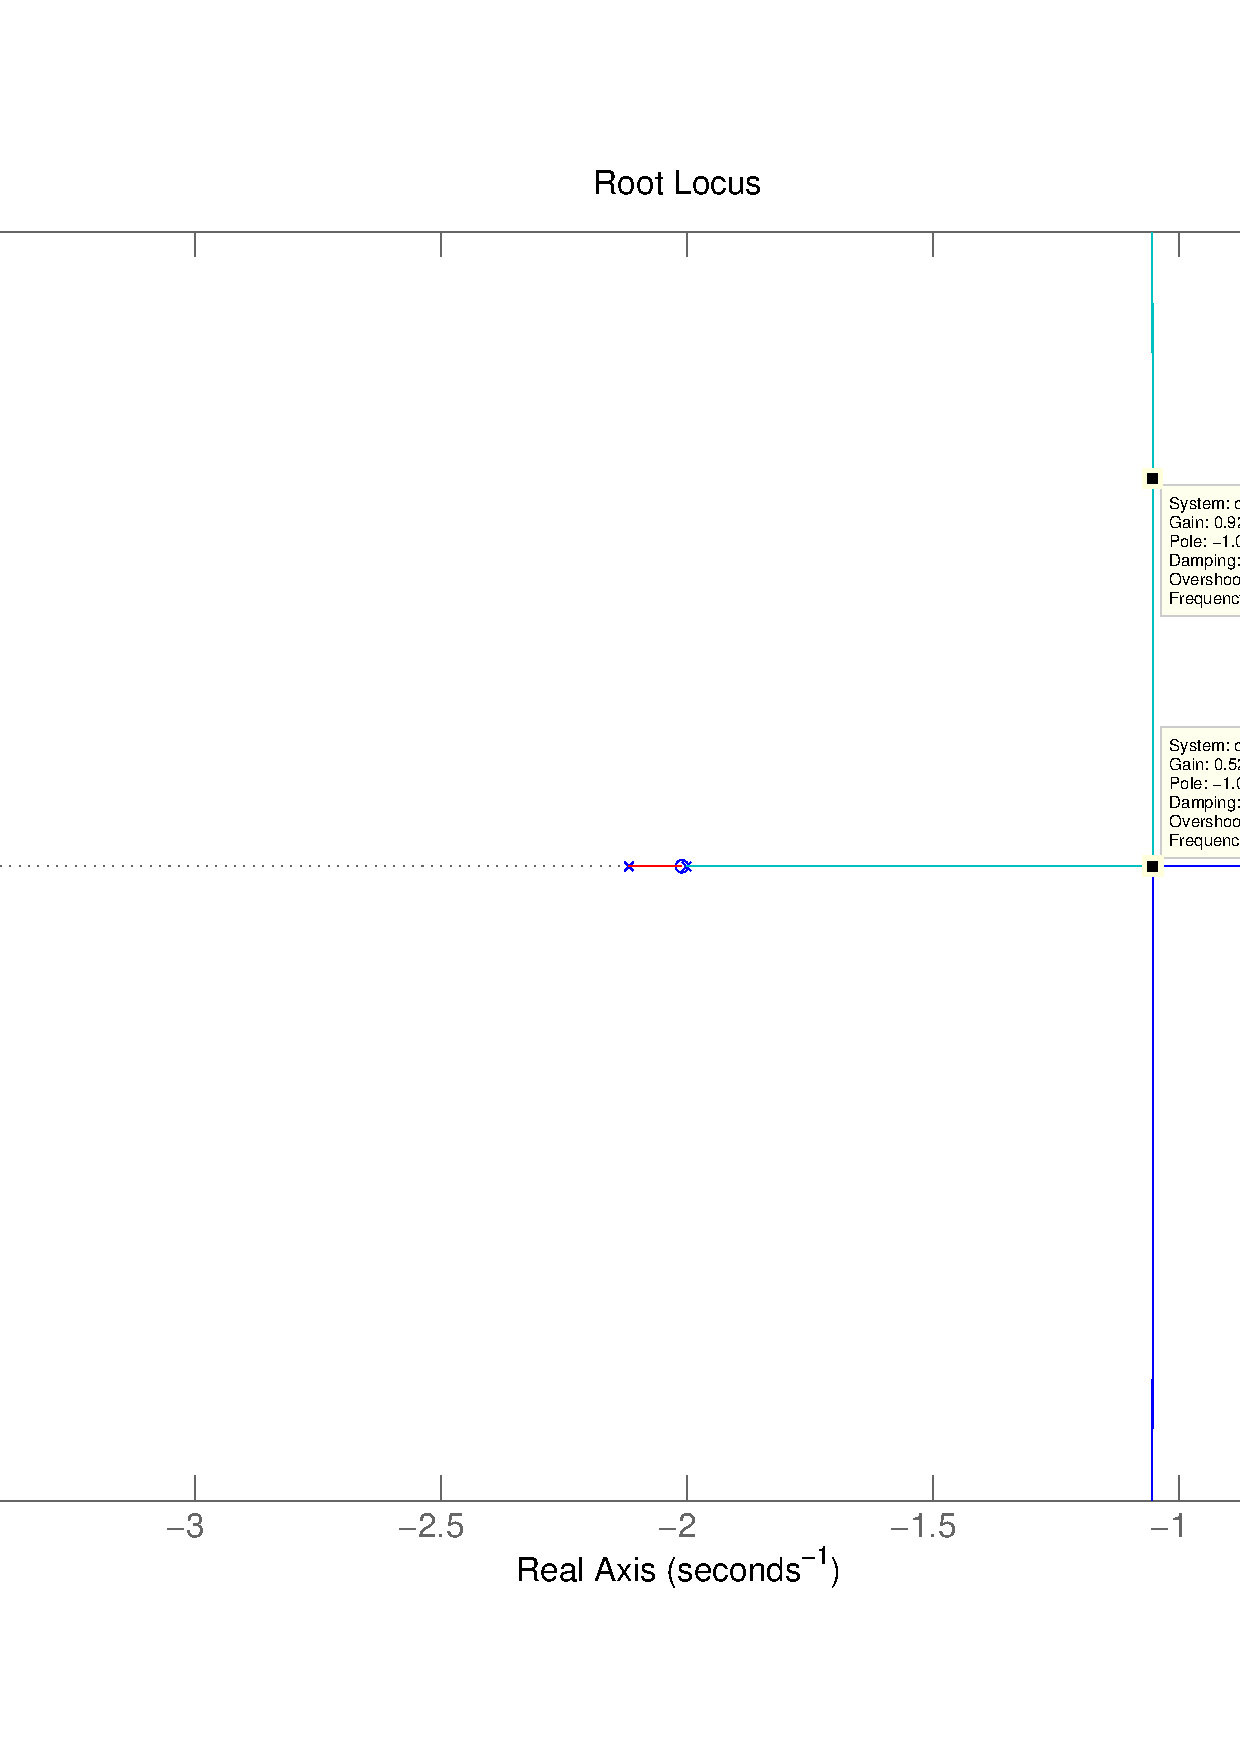
\includegraphics[width = \textwidth]{rlocus_outerTrac.pdf}
\end{frame}

\begin{frame}{Traction Control}
\framesubtitle{Simulation}
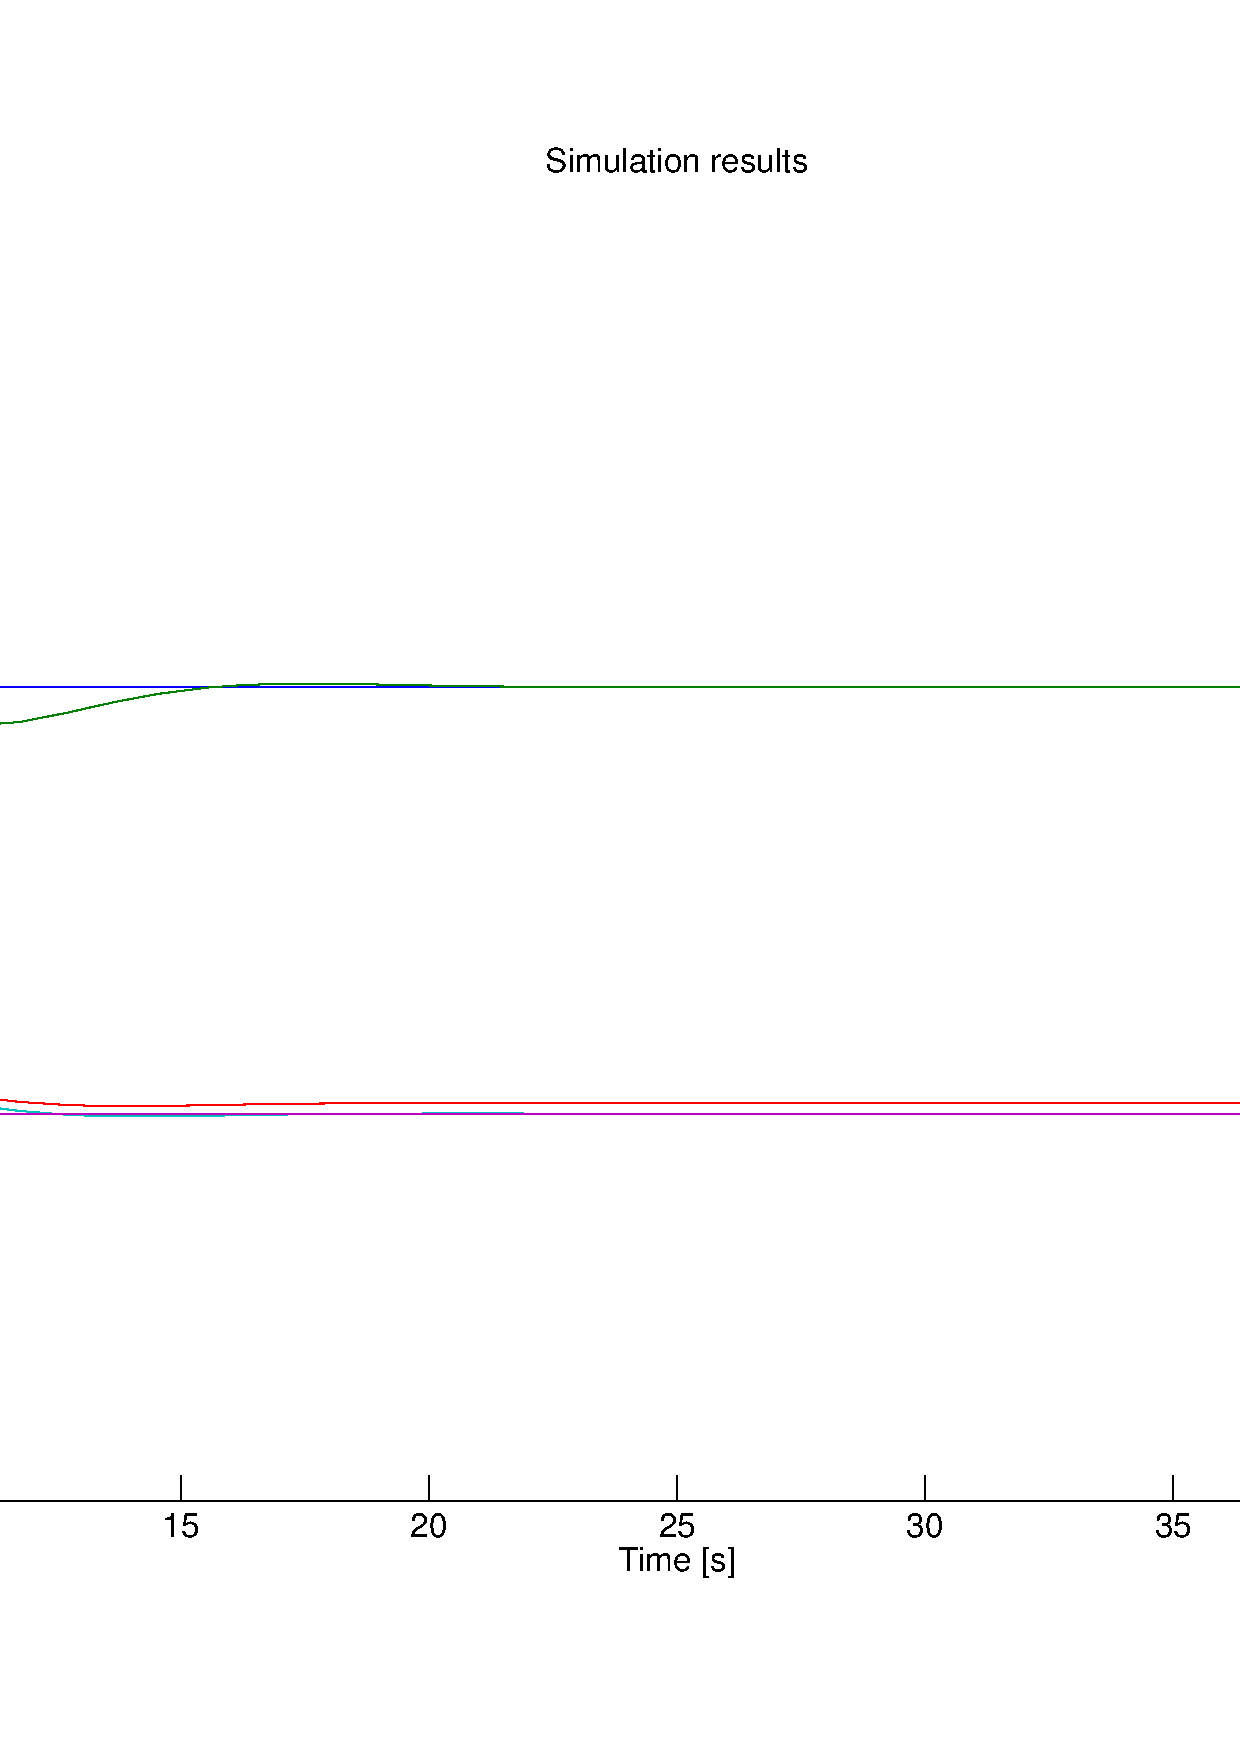
\includegraphics[width = \textwidth]{simu_tot_k06.pdf}\\
High overshoot\\$\Rightarrow$ should be primary tuning constraint
\end{frame}

\begin{frame}{Traction Control}
\framesubtitle{Final Controller Values}
\includegraphics[width = \textwidth]{totalOut_k_2_t_3_ramp.pdf}
\end{frame}

\begin{frame}{Traction Control}
\framesubtitle{Verification: Actuator Input}
\centering
\includegraphics[height = 0.8\textheight]{totalCurr_k_2_t_3_ramp.pdf}
\end{frame}





